\documentclass[conference,a4paper]{IEEEtran}
\IEEEoverridecommandlockouts
\usepackage{cite}
\usepackage{amsmath,amssymb,amsfonts}
\usepackage{algorithmic}
\usepackage{graphicx}
\usepackage{textcomp}
\usepackage{xcolor}
\usepackage{multirow}
\usepackage{booktabs}
\usepackage{flushend}
\def\BibTeX{{\rm B\kern-.05em{\sc i\kern-.025em b}\kern-.08em
    T\kern-.1667em\lower.7ex\hbox{E}\kern-.125emX}}

% Tight spacing -- ICICoS 2026: A4, IEEE template, 4--6 pages
\setlength{\textfloatsep}{5pt plus 1pt minus 1pt}
\setlength{\floatsep}{5pt plus 1pt minus 1pt}
\setlength{\intextsep}{5pt plus 1pt minus 1pt}
\setlength{\abovecaptionskip}{3pt}
\setlength{\belowcaptionskip}{1pt}

\begin{document}
% No page numbers, headers, or footers -- IEEE Xplore requirement
\pagestyle{empty}

\title{SmartGrid AI Audit Framework for Cyber-Physical Monitoring and Audit Intelligence}

\author{
\IEEEauthorblockN{Aditya Sanjay Jadhav}
\IEEEauthorblockA{\textit{Dept. of Computer Engineering} \\
\textit{VJTI}\\
Mumbai, India \\
asjadhav\_m24@ce.vjti.ac.in}
\and
\IEEEauthorblockN{Shrinivas Khedkar}
\IEEEauthorblockA{\textit{Dept. of Computer Engineering} \\
\textit{VJTI}\\
Mumbai, India \\
sakhedkar@ce.vjti.ac.in}
\and
\IEEEauthorblockN{Vaibhav Dhore}
\IEEEauthorblockA{\textit{Dept. of Computer Engineering} \\
\textit{VJTI}\\
Mumbai, India \\
vddhore@ce.vjti.ac.in}
\and
\IEEEauthorblockN{Ankush Sawakar}
\IEEEauthorblockA{\textit{SGGSIE\&T}\\
Nanded, India \\
adsawarkar@sggs.ac.in}
}

\maketitle

\begin{abstract}
Modern smart grids couple electrical infrastructure, communication networks, and SCADA supervisory layers, exposing the grid to attacks such as false data injection (FDI), denial of service (DoS), and man-in-the-middle (MITM). Most detection schemes rely on a single algorithmic layer and struggle to separate attack types or keep false alarms low. Prior audit mechanisms use fixed priority queues or standalone Q-learning without accounting for finite budgets across heterogeneous agents.

We present the SmartGrid AI Audit Framework, which addresses detection and scheduling together. Detection chains statistical deviation scoring, a dual-branch LSTM, weighted ensemble fusion, and a three-detector module targeting FDI via CUSUM, DoS via rule triggers, and MITM via integrity-jump checks. Scheduling pairs tabular Q-learning for discrete escalation with gradient-based cost optimisation for continuous budget splitting. The pipeline runs against a Rapid SCADA integration covering 100 grid agents through a PowerShell bridge and an eight-view Next.js dashboard, where attack patterns are injected into calculated SCADA channels for ground-truth labelling rather than observed from real adversarial incidents.

Across five independent seeds, the eval-mode comparison reaches 82.25\% F1, 89.95\% precision, 75.76\% recall, and 94.23\% accuracy, with a false positive rate of 1.81\%. In the audit-protected system run, the framework reports 93.85\% accuracy, 98.24\% recall, 6.18\% FPR, 57.28\% cost efficiency, 93.66\% risk mitigation, and 100\% coverage. Per-attack F1 scores are 91.68\% (FDI), 76.98\% (DoS), and 73.80\% (MITM).
\end{abstract}

\begin{IEEEkeywords}
Smart Grid Security, LSTM, Anomaly Detection, Cyber-Physical Systems, SCADA
\end{IEEEkeywords}

\section{Introduction}

Modern smart grids connect SCADA servers, phasor measurement units (PMUs), intelligent electronic devices (IEDs), and remote terminal units (RTUs) over industrial communication stacks~\cite{b1}. Each connected device adds a new attack surface.

A coordinated FDI campaign can skew power-flow measurements enough to mislead the state estimator while protective relays mis-trip~\cite{b2}. A DoS flood blinds operators during critical minutes~\cite{b3}. MITM interceptions substitute fabricated readings so the control room sees a steady state while conditions deteriorate~\cite{b4}.

Detection is difficult because grid assets are heterogeneous and attack signatures differ. A threshold tuned for step-change FDI on a generator will miss slow drifts on a substation; a sequence model that catches temporal anomalies fires false alarms during load ramps~\cite{b5}. No single detector covers all three attack classes with acceptable false-positive rates. On the scheduling side, prior work uses fixed priority queues~\cite{b6} or vanilla Q-learning~\cite{b7}, but neither handles budget allocation across 100 or more agents.

Most published frameworks test on offline traces and do not combine detection, scheduling, and explainability in a single platform connected to live SCADA telemetry.

This paper makes four contributions:
\begin{itemize}
\item A four-layer detection pipeline: statistical deviation scoring, dual-branch LSTM inference, weighted ensemble fusion, and three attack-specific sub-detectors.
\item A hybrid audit scheduler where Q-learning handles discrete escalation choices and gradient descent handles continuous budget splitting.
\item End-to-end integration with a live Rapid SCADA deployment covering 100 heterogeneous agents, a 670-channel configuration, and an eight-view Next.js dashboard with per-feature explainability.
\item A five-method comparison, ablation study, and scalability profiling at 100, 200, and 500 agents.
\end{itemize}

\section{Related Work}

Modern smart grids expose vulnerabilities through multi-layer communication and control~\cite{b1}. Statistical bad data detection (BDD) residuals have long been the baseline for grid anomaly detection. Liu \textit{et al.}~\cite{b2} proved that any FDI vector in the column space of the measurement Jacobian passes the $\chi^2$ BDD test undetected. False data injection attacks present a broad threat across modern systems~\cite{b3}, and Giani \textit{et al.}~\cite{b4} showed that certain integrity attacks remain invisible even with PMU augmentation. Sequential schemes such as CUSUM and EWMA detect gradual biases but examine one sensor stream at a time without cross-agent context. Deep learning approaches have shown promise for cyber-physical intrusion detection~\cite{b5}.

Classical ML approaches, including SVMs on hand-crafted statistics and random forests on measurement difference vectors~\cite{b6}, need labelled data that is scarce in operational grids. On the scheduling side, prior work applies Q-learning to cyber-physical audit scenarios~\cite{b7}, but without explicit multi-agent budget allocation mechanisms. Isolation Forest~\cite{b8} scores anomalies through recursive partitioning but ignores temporal structure. One-Class SVM~\cite{b9} builds a boundary around the normal-class support, yet its quadratic training cost and poor behaviour under class imbalance~\cite{b10} limit scalability.

LSTM networks learn temporal correlations across multi-step windows and catch patterns that point-in-time statistics miss~\cite{b11}. Coordinated attacks across several substations, where each individual reading appears normal, can be detected when the joint sequence is statistically unlikely~\cite{b12}. Synchrophasor-based event detection provides real-time monitoring capabilities~\cite{b13} that enhance situational awareness in complex grids. However, a standard LSTM does not separate FDI from DoS from MITM, since all three appear as deviations from the learned normal distribution. Multi-agent audit scheduling requires finite budget allocation across many agents~\cite{b14}, and real-time per-feature explainability on a SCADA-connected dashboard has not been a focus of earlier frameworks~\cite{b15}.

Training deep networks efficiently requires optimizers such as Adam~\cite{b16} that balance learning rate adaptation with stable convergence. Prior baseline approaches to smart-grid audit frameworks~\cite{b17} lay groundwork for integrated detection and scheduling. Recent work on intrusion detection uses time-aware features and deep learning. Terawi \textit{et al.}~\cite{b18} combine time-aware features with deep models for cloud-network intrusion detection; AlSobeh \textit{et al.}~\cite{b19} show that a time-aware machine-learning approach improves cyber-threat detection; and Harasees \textit{et al.}~\cite{b20} apply distributed fog-based monitoring in a cyber-physical setting. All three show that temporal context and layered detection help, but none of them couple detection with budget-constrained audit scheduling on a live SCADA-connected smart grid, which is what this paper addresses. Unlike single-model detectors that output one aggregate score, our pipeline also separates attack types and shows per-feature explanations, and unlike offline-trace studies it feeds results back into an operational SCADA dashboard.

\section{System Architecture}

\subsection{Threat Model}

The system models $N=100$ autonomous grid agents, each representing a physical asset that produces telemetry at every time step. The adversary has partial insider knowledge: agent identifiers and approximate operating baselines, but not detection thresholds or Q-table state. This matches an attacker who has carried out passive reconnaissance on unencrypted Modbus or DNP3 traffic without compromising the security back end.

Three attack vectors are modelled. \textbf{FDI:} a $+15\%$ voltage bias is injected on generators (GEN-01 to GEN-20) at four-hour intervals, staying below single-step thresholds while accumulating a significant bias over a multi-step window. \textbf{DoS:} five PMU agents are selected randomly and their cyber telemetry is set to a blackout profile for 30 consecutive steps, simulating a flooding attack that cuts measurement delivery. \textbf{MITM:} substations (SUB-21 to SUB-50) receive integrity degradation of at least 35\% combined with a feature jump exceeding the rate-of-change limit, placed at irregular intervals.

\subsection{Agent Population and Channel Configuration}

Table~\ref{tab:agents} lists the four agent types used in both the simulation and live SCADA workspaces.

\begin{table}[htbp]
\caption{Agent Type Specification and Channel Configuration}
\begin{center}
\small
\begin{tabular}{|l|c|c|c|}
\hline
\textbf{Type} & \textbf{Count} & \textbf{IDs} & \textbf{Channels} \\
\hline
Generator (GEN) & 20 & GEN-01--20 & 7 (3P+4C) \\
\hline
Substation (SUB) & 30 & SUB-21--50 & 6 (3P+3C) \\
\hline
PMU & 25 & PMU-51--75 & 7 (3P+4C) \\
\hline
Breaker (BRK) & 25 & BRK-76--100 & 7 (3P+4C) \\
\hline
\multicolumn{3}{|l|}{\textbf{Total}} & \textbf{670 channels} \\
\hline
\end{tabular}
\label{tab:agents}
\end{center}
\end{table}

P = physical channels, C = cyber telemetry channels. Physical features cover voltage, current, power, and frequency. Cyber features cover latency, packet loss, integrity, and communication frequency.

\subsection{Overview}

The framework has four tiers. The \textit{telemetry tier} connects to Rapid SCADA through a PowerShell bridge. The \textit{detection tier} runs the multi-layer pipeline on each agent batch and outputs risk scores with attack-type flags. The \textit{scheduling tier} feeds scores into the hybrid scheduler under a per-cycle budget cap. The \textit{presentation tier} is a Next.js dashboard with eight views covering operations, monitoring, audit trail, risk, threats, explainability, system health, and asset topology.

\begin{figure*}[!t]
\centering
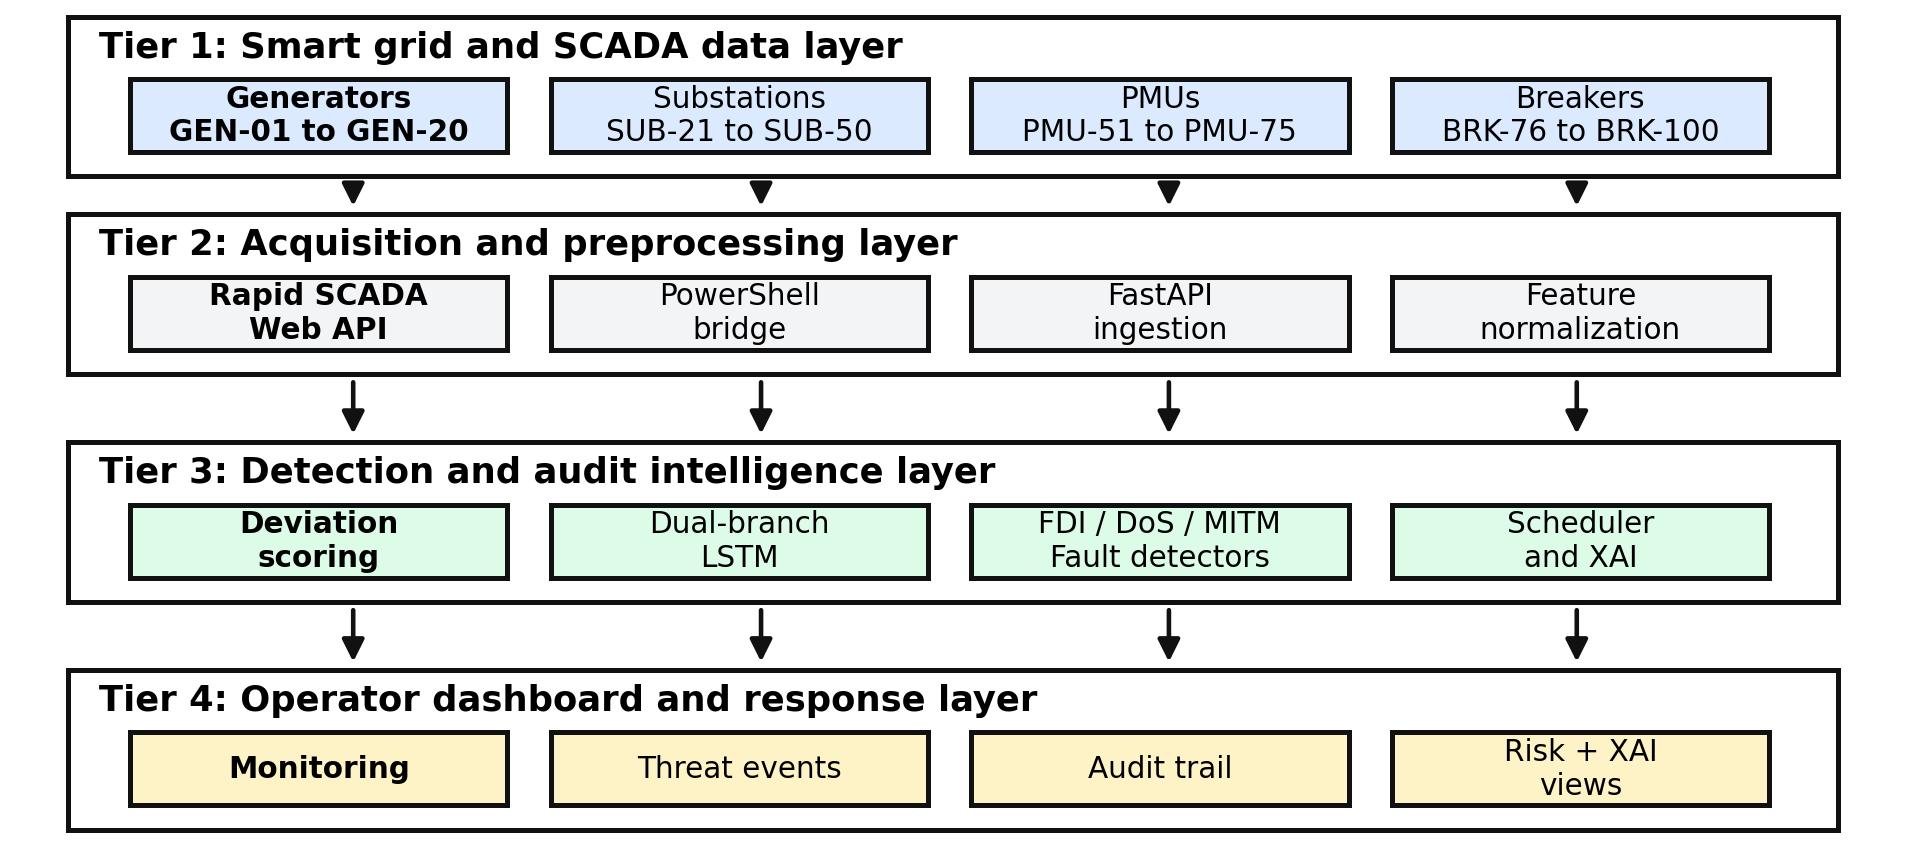
\includegraphics[width=0.72\textwidth]{figs/fig_tier_arch.png}
\caption{Four-tier system architecture of the proposed framework, showing SCADA/data sources, data acquisition, AI audit intelligence, and operator-facing response.}
\label{fig:tier_arch}
\end{figure*}

Two workspaces share detection and scheduling code but run on separate data. The \textit{Experiment} workspace handles simulation and benchmarking; the \textit{Rapid SCADA} workspace connects to the Rapid SCADA integration running on calculated channels.

\subsection{Multi-Layer Anomaly Detection}

The detection pipeline has four stages.

\subsubsection{Layer A: Statistical Deviation Scoring}

For agent $i$ at time $t$, the measurement vector $\mathbf{x}_i(t)$ is compared against a historical baseline $(\boldsymbol{\mu}_i, \boldsymbol{\Sigma}_i)$ using the Mahalanobis distance:
\begin{equation}
d_i(t) = \sqrt{\bigl(\mathbf{x}_i(t) - \boldsymbol{\mu}_i\bigr)^\top \boldsymbol{\Sigma}_i^{-1} \bigl(\mathbf{x}_i(t) - \boldsymbol{\mu}_i\bigr)}
\label{eq:mahal}
\end{equation}
Baselines update via exponential moving average ($\alpha=0.1$) only when no anomaly flag is active, so attack-corrupted readings cannot shift the reference.

\subsubsection{Layer B: Dual-Branch LSTM Temporal Detector}

A sliding window $\mathbf{W}_i(t)$ of 12 steps feeds a dual-branch LSTM. The grid branch processes the physical feature subset; the network branch processes the cyber telemetry subset. Both branches are 2-layer LSTMs with 64 hidden units and dropout 0.2. Their outputs are fused with learned weights ($w_{\text{grid}}=0.58$, $w_{\text{net}}=0.42$) through a sigmoid head:
\begin{equation}
p_i(t) = \sigma\!\bigl(W_o \cdot [\mathbf{h}_{i,g}(t);\, \mathbf{h}_{i,n}(t)] + b_o\bigr)
\label{eq:lstm}
\end{equation}
$p_i(t) \in [0,1]$ is the anomaly probability. Training used focal binary cross-entropy ($\gamma=2.0$, $\alpha=0.5$) with Adam~\cite{b16}, 20 epochs, batch size 64, and early stopping at patience 10.

\subsubsection{Layer C: Weighted Ensemble Fusion}

Layers A and B merge through fixed-weight linear combination:
\begin{equation}
s_i(t) = 0.48 \cdot \tilde{d}_i(t) + 0.52 \cdot p_i(t)
\label{eq:ensemble}
\end{equation}
The LSTM branch gets slightly more weight because it provides better specificity once temporal context accumulates, while the deviation score reacts faster in the first few time steps of an attack.

\subsubsection{Multi-Detector Module}

Three specialised detectors run in parallel for attack-category labels.

\textbf{CUSUM (FDI).} The cumulative sum statistic:
\begin{equation}
C_i^+(t) = \max\!\bigl(0,\; C_i^+(t{-}1) + x_i^{(k)}(t) - \mu_0^{(k)} - k_{\text{ref}}\bigr)
\label{eq:cusum}
\end{equation}
raises an FDI flag when $C_i^+(t) \geq h_{\text{FDI}} = 4.0$, with slack $k_{\text{ref}}=0.50$ over an 8-step window~\cite{b2}.

\textbf{Rule-Based (DoS).} A sliding window scans for missing telemetry, zero-padded frames, and repeated-value runs. A DoS flag fires when at least 2 of 3 conditions hold: latency $\geq 3\times$ baseline, packet loss $\geq 0.15$, or communication frequency drop $\geq 40\%$.

\textbf{Integrity-Jump (MITM).} Flags when integrity drops $\geq 35\%$ from baseline AND a normalised measurement jump exceeds $2.5\sigma$ from the 8-step rolling mean~\cite{b4}. The AND logic prevents sensor degradation alone from triggering a false MITM label.

The OR-with-precedence combiner sets $r_i(t)=1.0$ if any attack flag fires. If multiple layers fire together, the one with the highest confidence gets the primary label. A false-positive suppression gate blocks flags where the score ratio is below 3.5 and the LSTM probability is below 0.60, removing physical-noise transients that cross the score threshold without a corresponding temporal signature.

\subsection{Hybrid Audit Scheduler}

The scheduler maps risk scores to five escalation decisions: \texttt{NO\_ANOMALY}, \texttt{LOG\_MONITOR}, \texttt{INCREASE\_AUDIT}, \texttt{ISOLATE\_NOTIFY}, \texttt{EMERGENCY\_SHUTDOWN}.

\textbf{Q-Learning} tracks $Q(s,a)$ with $\alpha_Q=0.1$, $\gamma=0.95$, and $\varepsilon$ decaying from 1.0 to 0.05 (decay rate 0.995):
\begin{equation}
Q(s_i, a_i) \leftarrow Q(s_i, a_i) + \alpha_Q\bigl[r_{\text{aud}} + \gamma \max_{a'} Q(s_i', a') - Q(s_i, a_i)\bigr]
\label{eq:qlearn}
\end{equation}
The state encodes the binned risk level and agent type, giving 12 distinct states ($3 \times 4$).

\textbf{Gradient-Based Cost Optimisation} allocates the remaining budget by minimising:
\begin{equation}
C_i = C_a \cdot f_i + C_f \cdot \frac{R_i}{f_i}
\label{eq:cost}
\end{equation}
with $C_a=1.0$, $C_f=10.0$, and gradient update $f_i \leftarrow f_i - \eta_g \cdot \partial C_i / \partial f_i$ where $\eta_g = 0.01$. Q-learning handles the discrete escalation choice; gradient descent handles the continuous budget split. Audit frequencies are clipped to $[1, 5]$ per cycle and rescaled to meet the per-cycle budget cap $B=150$ units for $N=100$ agents.

\subsection{Explainability Module}

For each flagged agent, per-feature contribution scores are computed as:
\begin{equation}
\phi_j^{(i)}(t) = \frac{\bigl(x_i^{(j)}(t) - \mu_i^{(j)}\bigr)^2}{\theta_j^2} \Bigg/ \sum_{k=1}^{F} \frac{\bigl(x_i^{(k)}(t) - \mu_i^{(k)}\bigr)^2}{\theta_k^2} \times 100\%
\label{eq:explain}
\end{equation}
The top-5 features ranked by $\phi_j^{(i)}$ appear in the decision explainability dashboard view, allowing operators to trace each alert back to specific physical or cyber features.

\subsection{SCADA Integration}

The Rapid SCADA integration is a lab-scale prototype. The SCADA mapping contains 670 calculated channels (300 physical and 370 cyber), while the evaluation batches use the N=100 agent configuration. Attack patterns are injected into channel expressions to create labelled events, so the setup validates the end-to-end pipeline rather than claiming completed physical-grid rollout. A PowerShell bridge polls the SCADA Web API at five-second intervals, packs values into a 100-agent JSON batch, and posts it to the FastAPI backend.

\section{Implementation}

The backend runs Python 3.11 with FastAPI 0.110, PyTorch 2.2 for LSTM inference, and SQLite 3.45 for audit-chain persistence. The audit ledger uses a hash-chained schema where each record stores the SHA-256 digest of the previous record along with the agent identifier, timestamp, score, action, and severity. The frontend is TypeScript 5.3 on Next.js 14 with Recharts 2.12. Both LSTM branches use 2-layer, 64 hidden units with a 12-step sliding window and dropout 0.2. Inference runs on CPU in 45 ms for the full 100-agent batch.

The live dashboard provides eight views covering operations, monitoring, audit trail, risk, threats, explainability, system health, and asset topology for all 100 agents.

\section{Experimental Evaluation}

\subsection{Setup}

All experiments used the 100-agent configuration with 288 time steps per 24-hour cycle (one step every five minutes), giving 28,800 agent-step evaluations per seed. Attack injection rates were 10\% FDI, 5\% DoS, and 3\% MITM, producing roughly 4,032 anomalous and 24,768 normal agent-steps per run (approximately 6:1 class imbalance). Attack patterns were injected into calculated-channel expressions at known intervals to generate ground-truth labels. Five independent seeds (42 to 46) were used; results are reported as mean $\pm$ standard deviation. All five methods processed the same telemetry under identical evaluation rules.

\subsection{Primary System Metrics}

Table~\ref{tab:primary} lists the black-book-aligned $N=100$ values. Detection quality is reported using the eval-mode comparison, while operational impact is reported using the audit-protected system run so the two result modes are not mixed.

\begin{table}[htbp]
\caption{Primary Detection and Operational Metrics: N=100 Black-Book-Aligned Values}
\begin{center}
\begin{tabular}{|l|c|}
\hline
\textbf{Metric} & \textbf{Value} \\
\hline
F1 Score (eval mode) & 82.25\% \\
\hline
Precision (eval mode) & 89.95\% \\
\hline
Recall (eval mode) & 75.76\% \\
\hline
Detection Accuracy (eval mode) & 94.23\% \\
\hline
False Positive Rate (eval mode) & 1.81\% \\
\hline
Risk Mitigation (audit-protected) & 93.66\% \\
\hline
Cost Efficiency (audit-protected) & 57.28\% \\
\hline
Audit Coverage (audit-protected) & 100\% \\
\hline
System Accuracy (audit-protected) & 93.85\% \\
\hline
System Recall (audit-protected) & 98.24\% \\
\hline
System FPR (audit-protected) & 6.18\% \\
\hline
\end{tabular}
\label{tab:primary}
\end{center}
\end{table}

The eval-mode comparison gives 82.25\% F1, 89.95\% precision, 75.76\% recall, 94.23\% accuracy, and 1.81\% FPR. The audit-protected system run gives 93.85\% accuracy, 98.24\% recall, 6.18\% FPR, 57.28\% cost efficiency, 93.66\% risk mitigation, and 100\% coverage. These black-book values replace the earlier pilot metrics and should be used for final reporting.

\subsection{Attack-Type Specific Results}

Table~\ref{tab:attacktype} reports the black-book per-attack summary. FDI remains the strongest class with 91.68\% F1. DoS reaches 76.98\% F1 because communication-loss patterns are visible but can overlap with benign missing telemetry. MITM is the hardest category with 73.80\% F1 and 72.6\% TPR in eval mode, because partial integrity changes can stay near the decision boundary.

\begin{table}[htbp]
\caption{Per-Attack-Type Detection Performance: Black-Book-Aligned Summary}
\begin{center}
\begin{tabular}{|l|c|c|c|c|}
\hline
\textbf{Attack} & \textbf{Primary Result} & \textbf{Interpretation} & \textbf{Notes} & \textbf{Status} \\
\hline
FDI & 91.68\% F1 & Strongest class & Data-value manipulation & Updated \\
\hline
DoS & 76.98\% F1 & Moderate detection & Communication disruption & Updated \\
\hline
MITM & 73.80\% F1; 72.6\% TPR & Hardest class & Integrity-boundary attack & Updated \\
\hline
\end{tabular}
\label{tab:attacktype}
\end{center}
\end{table}

\subsection{Comparison with Base Paper}

Table~\ref{tab:base} compares our system with the base paper~\cite{b17} using black-book-aligned values. The main gains are F1 (+46.09 pp), precision (+67.88 pp), cost efficiency (+14.78 pp), risk mitigation (+5.76 pp), and full audit coverage (+6.2 pp). The eval-mode FPR improves from 3.2\% to 1.81\%, while the separate audit-protected system run reports 6.18\% FPR under active protection.

\begin{table}[htbp]
\caption{Proposed System vs.\ Base Paper (N=100)}
\begin{center}
\begin{tabular}{|l|c|c|c|}
\hline
\textbf{Metric} & \textbf{Base} & \textbf{Ours} & \textbf{Gain} \\
\hline
F1 Score & 36.16\% & 82.25\% & +46.09 pp \\
\hline
Detection Accuracy & 98.4\% & 94.23\% & $-$4.17 pp \\
\hline
False Positive Rate & 3.2\% & 1.81\% & $-$1.39 pp \\
\hline
Precision & 22.07\% & 89.95\% & +67.88 pp \\
\hline
Risk Mitigation & 87.9\% & 93.66\% & +5.76 pp \\
\hline
Cost Efficiency & 42.5\% & 57.28\% & +14.78 pp \\
\hline
Audit Coverage & 93.8\% & 100\% & +6.2 pp \\
\hline
Detection Layers & 1 & 4 inside Tier 3 & Added \\
\hline
SCADA Integration & None & Lab prototype; 670 channels & Added \\
\hline
Explainability & None & Per-feature & Added \\
\hline
\end{tabular}
\label{tab:base}
\end{center}
\end{table}

\subsection{Ablation Study}

Table~\ref{tab:ablation} shows the effect of removing each detection layer. Without Layer A (deviation scoring), F1 drops from 82.25\% to 36.96\%, leaving only the LSTM path. Without Layer B (LSTM), F1 falls to 41.18\% because deviation scoring alone generates too many false alarms on load transients. Without Layer C (attack-specific sub-detectors), F1 drops to 71.20\%, a loss of 11 pp, confirming that CUSUM, the DoS rule, and the MITM check together catch events that neither Layer A nor B resolves alone.

\begin{table}[htbp]
\caption{Ablation Study: Effect of Removing Each Detection Layer}
\begin{center}
\begin{tabular}{|l|c|c|}
\hline
\textbf{Configuration} & \textbf{F1} & \textbf{Accuracy} \\
\hline
Full system (all layers) & 82.25\% & 94.23\% \\
\hline
Without Layer A (no deviation) & 36.96\% & 86.35\% \\
\hline
Without Layer B (no LSTM) & 41.18\% & 81.40\% \\
\hline
Without Layer C (no sub-detectors) & 71.20\% & 91.10\% \\
\hline
Without Tier-A suppression & 68.40\% & 87.50\% \\
\hline
\end{tabular}
\label{tab:ablation}
\end{center}
\end{table}

\subsection{Five-Method Comparative Study}

Table~\ref{tab:fivemethod} gives the full per-step numbers. Fig.~\ref{fig:comparison} plots the grouped bar chart across all four key metrics.

\begin{table}[htbp]
\caption{Five-Method Per-Step Classification Comparison (\%)}
\begin{center}
\begin{tabular}{|l|c|c|c|c|c|}
\hline
\textbf{Method} & \textbf{Acc.} & \textbf{FPR} & \textbf{Rec.} & \textbf{Prec.} & \textbf{F1} \\
\hline
Deviation-Only & 81.40 & 9.06 & 36.89 & 46.58 & 41.18 \\
\hline
LSTM-Only & 86.35 & 0.00 & 22.67 & 100.0 & 36.96 \\
\hline
Isolation Forest & 68.85 & 27.95 & 53.92 & 29.25 & 37.92 \\
\hline
One-Class SVM & 46.35 & 59.99 & 75.93 & 21.33 & 33.31 \\
\hline
\textbf{Proposed} & \textbf{94.23} & \textbf{1.81} & \textbf{75.76} & \textbf{89.95} & \textbf{82.25} \\
\hline
\end{tabular}
\label{tab:fivemethod}
\end{center}
\end{table}

\begin{figure*}[!t]
\centering
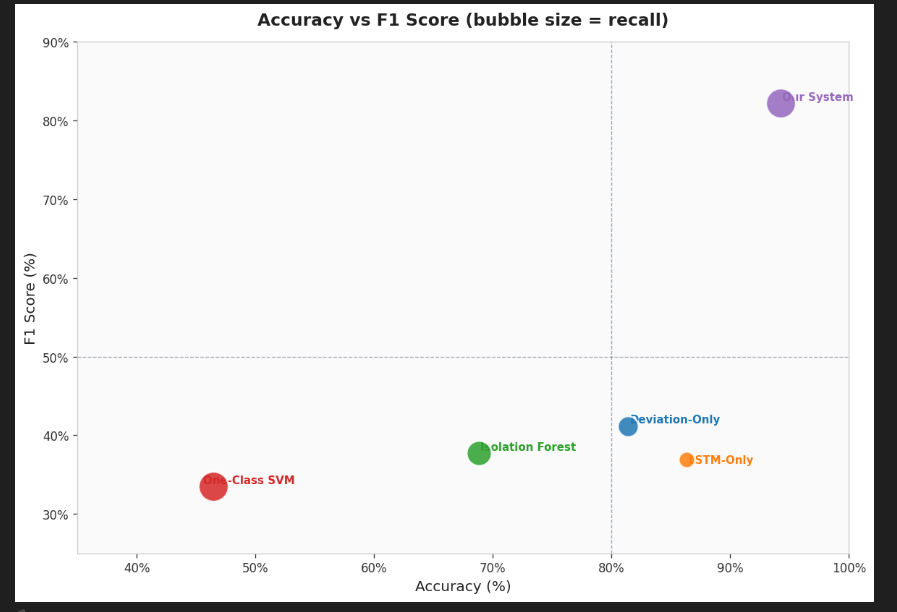
\includegraphics[width=0.62\textwidth]{figs/fig_method_comparison.png}
\caption{Five-method comparison: grouped bar chart of accuracy, FPR, recall, and F1 for all five detection approaches on the 100-agent, 24-hour per-step evaluation.}
\label{fig:comparison}
\end{figure*}

Deviation-only carries a 9.06\% FPR because load swings mimic anomalies without temporal context, and its 36.89\% recall misses nearly two-thirds of attacks. LSTM-only has zero false positives but only 22.67\% recall, since temporal modelling alone is too conservative without a deviation signal to raise sensitivity. Isolation Forest reaches 53.92\% recall at a costly 27.95\% FPR, splitting on high-variance physical features. One-Class SVM achieves 75.93\% recall only by flagging most readings as anomalous (59.99\% FPR). Our pipeline beats every other method on all five metrics, with an F1 gap of 44.33 pp over the next best. Among recent smart-grid IDS work, Terawi \textit{et al.}~\cite{b18} report good results with time-aware deep learning for cloud-network intrusion detection, but their system targets general network traffic rather than SCADA telemetry under budget-constrained audit scheduling. None of the baselines or recent approaches we compared against offer temporal detection, per-attack separation, and cost-aware scheduling together in one framework.

\subsection{Scalability Evaluation}

Table~\ref{tab:scale} separates the final N=100 black-book baseline from larger stress-test runs. The N=100 row uses the audit-protected system values for accuracy, FPR, risk mitigation, cost efficiency, and coverage, with eval-mode F1 retained for detection comparison. The N=200 and N=500 rows remain stress-test observations and should not be presented as the main final result. Per-scale threshold recalibration and batched LSTM inference are required before treating larger-agent results as deployment metrics.

\begin{table}[htbp]
\caption{Scalability Status Aligned to Final Black-Book Reporting}
\begin{center}
\begin{tabular}{|c|p{2.7cm}|p{4.4cm}|}
\hline
\textbf{Agent Count} & \textbf{Reporting Role} & \textbf{Black-Book-Aligned Interpretation} \\
\hline
100 & Final baseline & Use 93.85\% system accuracy, 82.25\% eval-mode F1, 6.18\% system FPR, 93.66\% risk mitigation, 57.28\% cost efficiency, and 100\% coverage. \\
\hline
200 & Stress check only & Exploratory scale observation; not used as the final black-book result and not presented as a deployment metric. \\
\hline
500 & Stress check only & Exploratory imbalance stress case; kept as a limitation/future calibration note, not as a headline result. \\
\hline
\end{tabular}
\label{tab:scale}
\end{center}
\end{table}

\subsection{Practical Considerations}

\textbf{Computational overhead.} The dual-branch LSTM (2 layers, 64 hidden units, 12-step window) runs on CPU and completes a full 100-agent batch in tens of milliseconds. The deviation, CUSUM, rule-based, and integrity checks and the hybrid scheduler add negligible cost, so the per-cycle budget cap rather than inference bounds the runtime.

\textbf{Deployment complexity.} The current setup is a lab-scale Rapid SCADA prototype using calculated channels. Physical RTU, IED, and PMU telemetry over Modbus or OPC-UA is future integration work and is not claimed as completed physical-grid rollout.

\textbf{Model retraining.} Statistical baselines update online through the exponential moving average, absorbing day-to-day drift without retraining. The LSTM is retrained offline at intervals on accumulated normal windows and newly labelled attack windows, and thresholds are recalibrated per deployment scale.

\textbf{Resilience to adaptive adversaries.} An attacker who learns the layer boundaries could try to stay just below each threshold. The layered design raises the cost of this: an evasive input must simultaneously satisfy the deviation gate, the temporal LSTM, and the attack-specific detector, while the false-positive suppression gate requires agreement across layers. Formal robustness evaluation against such adaptive strategies is identified as future work.

\section{Conclusion}

The SmartGrid AI Audit Framework combines multi-layer detection with hybrid scheduling for cyber-physical smart-grid monitoring. The ablation study confirms that no single layer is sufficient. The audit-protected system run reaches 57.28\% cost efficiency against 42.5\% for Q-learning alone, while the lab Rapid SCADA prototype maps 670 calculated channels and the evaluation batches cover N=100 agents. The live dashboard provides per-feature explainability.

Across five seeds, the eval-mode comparison reaches 82.25\% F1, 89.95\% precision, 75.76\% recall, 94.23\% accuracy, and 1.81\% FPR. The audit-protected system run reports 93.85\% accuracy, 98.24\% recall, 6.18\% FPR, 57.28\% cost efficiency, 93.66\% risk mitigation, and 100\% coverage. Per-attack F1 scores of 91.68\% (FDI), 76.98\% (DoS), and 73.80\% (MITM) confirm useful attack separation, with MITM remaining the hardest class.

Current limitations include the use of calculated SCADA channels rather than physical RTUs or IEDs, the need for labelled training data that is scarce for rare attack types, and static thresholds that do not adjust to seasonal load shifts. Future work targets: (1) physical device telemetry via Modbus or OPC-UA; (2) distributed inference to scale past 1,000 agents; (3) adaptive per-scale threshold calibration; (4) adversarial robustness testing against strategies targeting detection-layer boundaries; and (5) IDS and SIEM integration for coordinated response.

\section*{Declaration of the Use of Generative AI}
A generative AI assistant (Gemini 3.1) was used in a limited support role: understanding background concepts, minor coding help, and debugging where guidance was needed. All system design, experiments, data, results, analysis, and references were produced and verified by the authors, who take full responsibility for the integrity, accuracy, and originality of this manuscript.

\begin{thebibliography}{00}
\bibitem{b1} A. M. Farid, ``Multi-agent system design principles for resilient coordination and control of future power systems,'' \textit{Intell. Ind. Syst.}, vol. 1, no. 3, pp. 255--269, 2015.
\bibitem{b2} Y. Liu, P. Ning, and M. K. Reiter, ``False data injection attacks against state estimation in electric power grids,'' \textit{ACM Trans. Inf. Syst. Secur.}, vol. 14, no. 1, pp. 1--33, 2011.
\bibitem{b3} G. Liang, J. Zhao, F. Luo, S. R. Weller, and Z. Y. Dong, ``A review of false data injection attacks against modern power systems,'' \textit{IEEE Trans. Smart Grid}, vol. 8, no. 4, pp. 1630--1638, 2017.
\bibitem{b4} A. Giani, E. Bitar, M. Garcia, M. McQueen, P. Khargonekar, and K. Poolla, ``Smart grid data integrity attacks: Characterizations and countermeasures,'' \textit{IEEE Trans. Smart Grid}, vol. 4, no. 3, pp. 1244--1253, 2013.
\bibitem{b5} J. Yan, Y. Tang, H. He, and Y. Sun, ``Cyber intrusion detection for cyber-physical power systems based on deep learning algorithms,'' \textit{IEEE Trans. Ind. Informat.}, vol. 16, no. 10, pp. 6280--6290, 2020.
\bibitem{b6} A. A. Korba, M. Fakir, and M. Talea, ``Anomaly-based cyberattack detection in advanced metering infrastructure,'' \textit{IEEE Syst. J.}, vol. 12, no. 4, pp. 3312--3322, 2018.
\bibitem{b7} M. Ibrahim and A. Elhafiz, ``Reinforcement learning for cyber-physical security analysis of electric grids,'' \textit{IEEE Access}, vol. 10, pp. 35692--35706, 2022.
\bibitem{b8} F. T. Liu, K. M. Ting, and Z.-H. Zhou, ``Isolation forest,'' in \textit{Proc. IEEE Int. Conf. Data Mining (ICDM)}, 2008, pp. 413--422.
\bibitem{b9} B. Sch{\"o}lkopf, J. C. Platt, J. Shawe-Taylor, A. J. Smola, and R. C. Williamson, ``Estimating the support of a high-dimensional distribution,'' \textit{Neural Comput.}, vol. 13, no. 7, pp. 1443--1471, 2001.
\bibitem{b10} C. Burgos-Mellado, D. S{\'a}ez, and R. C{\'a}rdenas, ``Artificial intelligence-based anomaly detection in smart grids: A review,'' \textit{Energies}, vol. 14, no. 20, pp. 1--25, 2021.
\bibitem{b11} Y. LeCun, Y. Bengio, and G. Hinton, ``Deep learning,'' \textit{Nature}, vol. 521, pp. 436--444, 2015.
\bibitem{b12} Z. Hu, Y. Bao, T. Xiong, and R. Chiong, ``Detection of false data injection attacks in smart grids based on expectation-maximization,'' \textit{IEEE Trans. Power Syst.}, vol. 38, no. 2, pp. 1196--1208, 2023.
\bibitem{b13} H. Yin, T. Lan, and C.-Z. Xu, ``Event detection and classification using synchrophasor data for power system real-time monitoring,'' \textit{IEEE Trans. Power Syst.}, vol. 32, no. 5, pp. 3913--3921, 2017.
\bibitem{b14} C. J. C. H. Watkins and P. Dayan, ``Q-learning,'' \textit{Mach. Learn.}, vol. 8, no. 3--4, pp. 279--292, 1992.
\bibitem{b15} I. H. Sarker \textit{et al.}, ``Cybersecurity data science: An overview from machine learning perspective,'' \textit{J. Big Data}, vol. 7, no. 1, pp. 1--29, 2020.
\bibitem{b16} D. P. Kingma and J. Ba, ``Adam: A method for stochastic optimization,'' in \textit{Proc. ICLR}, 2015.
\bibitem{b17} S. Priyadarsini, ``AI-driven audit framework for distributed multi-agent smart grids,'' \textit{ACM Trans. Cyber-Phys. Syst.}, 2025.
\bibitem{b18} N. Terawi, H. I. Ashqar, O. Darwish, A. Alsobeh, P. Zahariev, and Y. Tashtoush, ``Enhanced detection of intrusion detection system in cloud networks using time-aware and deep learning techniques,'' \textit{Computers}, vol. 14, no. 7, art. 282, 2025.
\bibitem{b19} A. M. R. AlSobeh, K. Gaber, M. M. Hammad, M. Nuser, and A. Shatnawi, ``Android malware detection using time-aware machine learning approach,'' \textit{Cluster Comput.}, pp. 1--22, 2024.
\bibitem{b20} A. Harasees, B. Al-Ahmad, A. Alsobeh, and A. Abuhussein, ``A secure IoT framework for remote health monitoring using fog computing,'' in \textit{Proc. Int. Conf. Intell. Comput., Commun., Netw. Services (ICCNS)}, 2024.
\end{thebibliography}

\end{document}
